\section{Back-test results}

In the $1/N$ strategy, on the first trading day we invest  an equal amount into each asset, and then leave the assets be for the entire trading period.

Since we are investing into 10 assets at a cost of 0.1\% of the trading volume, it costs us 1000 DKK to make the initial trade.
The remaining 999.000 DKK are left to grow during the entire period.

This strategy yields an annualized return of 5.7\% for the max-mean assets, and of 2.4\% for the min-stdev.


\begin{figure}[tp]
\centering
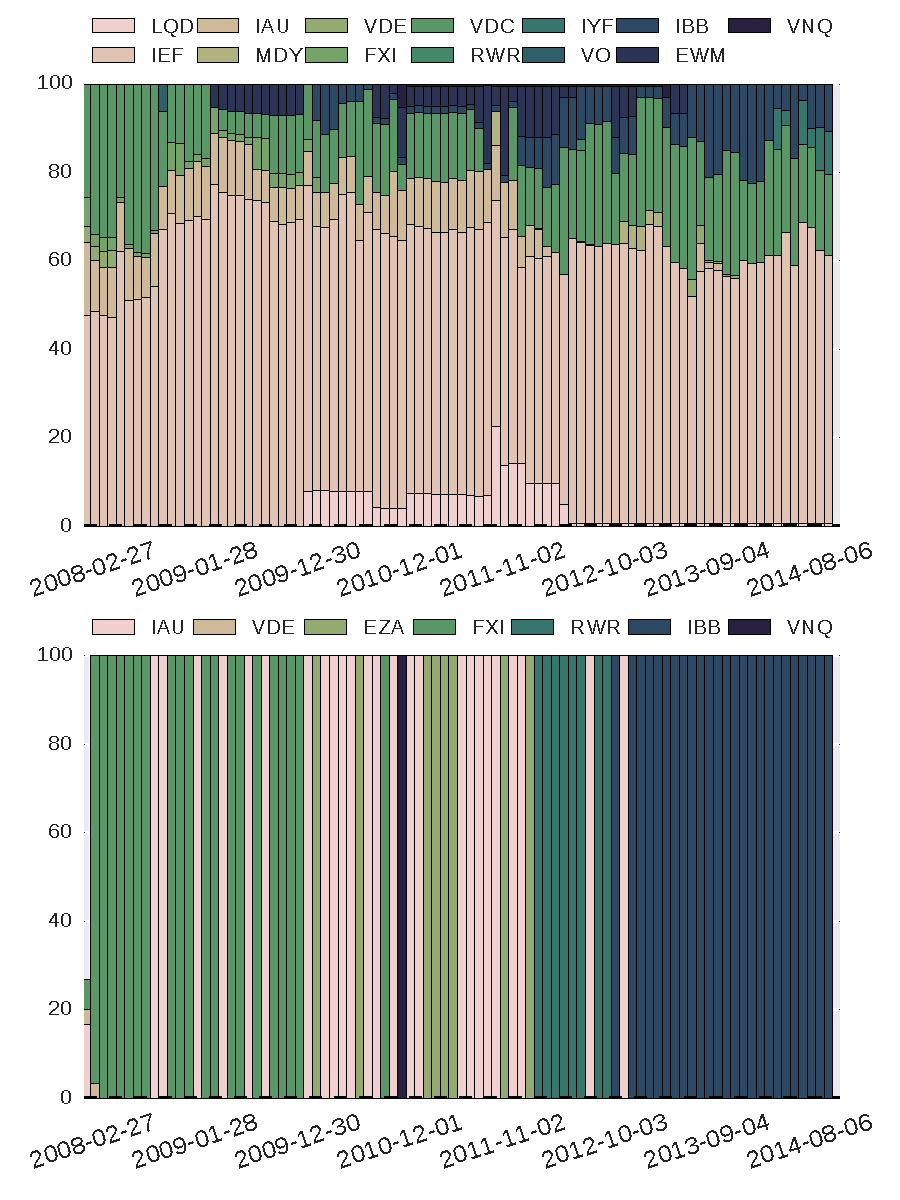
\includegraphics{../pic/trading_portfolio.pdf}
\caption{Portfolios found by the risk-averse (top) and risk-neutral (bottom) trading strategies.}
\label{fig:tradingportfolios}
\end{figure}


\begin{figure}[tp]
\centering
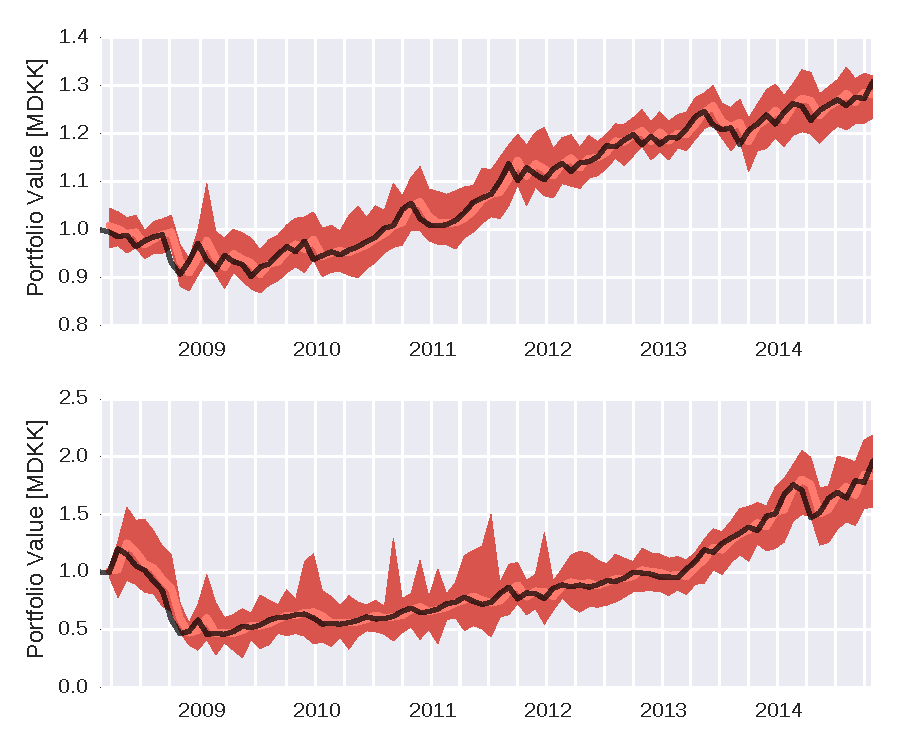
\includegraphics{../pic/trading_forecasted_value.pdf}
\caption{Nominal values of portfolios over time (Black line) versus forecasted mean value (light red). The shaded region indicates the maximum and minimum forecasted values of the ensembles.}
\label{fig:tradingforecastedvalues}
\end{figure}

\begin{figure}[tp]
\centering
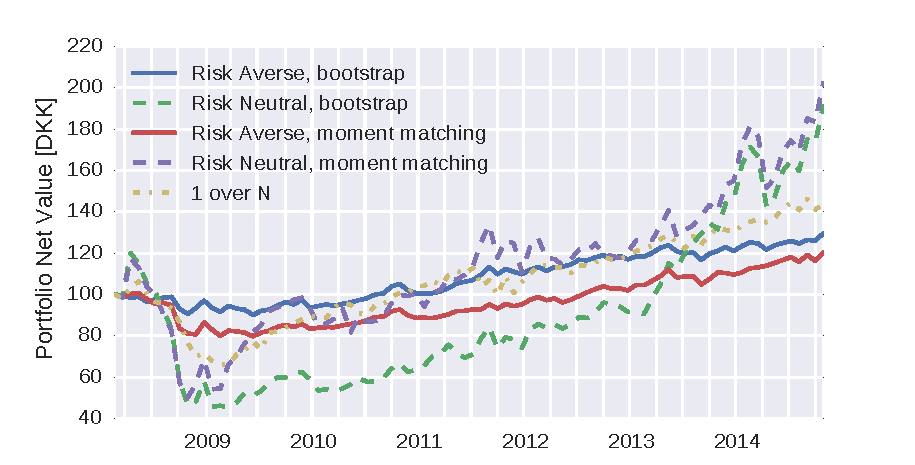
\includegraphics{../pic/trading_portfolio_value.pdf}
\caption{Net values of portfolios over time. (Net value = nominal value minus cumulative trading costs)}
\label{fig:tradingportfoliovalues}
\end{figure}

\begin{table}
\caption{Comparison of trading strategies}\label{tbl:portfoliotabel}
\centering
\begin{tabular}{lrrrl}
\toprule
{} & Final Nominal &  Trading &  Final Net & Annualized \\
{} & Value & Costs & Profit & Return \\
\midrule
Risk Averse, bootstrap        &              1259714 &          10810 &            248904 &             3.6 \% \\
Risk Neutral, bootstrap       &              1639882 &          43283 &            596599 &             7.7 \% \\
Risk Averse, moment matching  &              1172530 &           5797 &            166733 &             2.5 \% \\
Risk Neutral, moment matching &              1701345 &           8787 &            692558 &             8.7 \% \\
1 over N                      &              1462676 &              0 &            462676 &             6.2 \% \\
\bottomrule
\end{tabular}

\end{table}